\documentclass[12pt,a4paper]{article}

\usepackage[in, plain]{fullpage}
\usepackage{array}
\usepackage{../../../pas-math}
\usepackage{../../../moncours}


%\usepackage{pas-cours}
%-------------------------------------------------------------------------------
%          -Packages nécessaires pour écrire en Français et en UTF8-
%-------------------------------------------------------------------------------
\usepackage[utf8]{inputenc}
\usepackage[frenchb]{babel}
\usepackage[T1]{fontenc}
\usepackage{lmodern}
\usepackage{textcomp}



%-------------------------------------------------------------------------------

%-------------------------------------------------------------------------------
%                          -Outils de mise en forme-
%-------------------------------------------------------------------------------
\usepackage{hyperref}
\hypersetup{pdfstartview=XYZ}
%\usepackage{enumerate}
\usepackage{graphicx}
\usepackage{multicol}
\usepackage{tabularx}
\usepackage{multirow}


\usepackage{anysize} %%pour pouvoir mettre les marges qu'on veut
%\marginsize{2.5cm}{2.5cm}{2.5cm}{2.5cm}

\usepackage{indentfirst} %%pour que les premier paragraphes soient aussi indentés
\usepackage{verbatim}
\usepackage{enumitem}
\usepackage[usenames,dvipsnames,svgnames,table]{xcolor}

\usepackage{variations}

%-------------------------------------------------------------------------------


%-------------------------------------------------------------------------------
%                  -Nécessaires pour écrire des mathématiques-
%-------------------------------------------------------------------------------
\usepackage{amsfonts}
\usepackage{amssymb}
\usepackage{amsmath}
\usepackage{amsthm}
\usepackage{tikz}
\usepackage{xlop}
%-------------------------------------------------------------------------------



%-------------------------------------------------------------------------------


%-------------------------------------------------------------------------------
%                    - Mise en forme avancée
%-------------------------------------------------------------------------------

\usepackage{ifthen}
\usepackage{ifmtarg}


\newcommand{\ifTrue}[2]{\ifthenelse{\equal{#1}{true}}{#2}{$\qquad \qquad$}}

%-------------------------------------------------------------------------------

%-------------------------------------------------------------------------------
%                     -Mise en forme d'exercices-
%-------------------------------------------------------------------------------
%\newtheoremstyle{exostyle}
%{\topsep}% espace avant
%{\topsep}% espace apres
%{}% Police utilisee par le style de thm
%{}% Indentation (vide = aucune, \parindent = indentation paragraphe)
%{\bfseries}% Police du titre de thm
%{.}% Signe de ponctuation apres le titre du thm
%{ }% Espace apres le titre du thm (\newline = linebreak)
%{\thmname{#1}\thmnumber{ #2}\thmnote{. \normalfont{\textit{#3}}}}% composants du titre du thm : \thmname = nom du thm, \thmnumber = numéro du thm, \thmnote = sous-titre du thm

%\theoremstyle{exostyle}
%\newtheorem{exercice}{Exercice}
%
%\newenvironment{questions}{
%\begin{enumerate}[\hspace{12pt}\bfseries\itshape a.]}{\end{enumerate}
%} %mettre un 1 à la place du a si on veut des numéros au lieu de lettres pour les questions 
%-------------------------------------------------------------------------------

%-------------------------------------------------------------------------------
%                    - Mise en forme de tableaux -
%-------------------------------------------------------------------------------

\renewcommand{\arraystretch}{1.7}

\setlength{\tabcolsep}{1.2cm}

%-------------------------------------------------------------------------------



%-------------------------------------------------------------------------------
%                    - Racourcis d'écriture -
%-------------------------------------------------------------------------------

% Angles orientés (couples de vecteurs)
\newcommand{\aopp}[2]{(\vec{#1}, \vec{#2})} %Les deuc vecteurs sont positifs
\newcommand{\aopn}[2]{(\vec{#1}, -\vec{#2})} %Le second vecteur est négatif
\newcommand{\aonp}[2]{(-\vec{#1}, \vec{#2})} %Le premier vecteur est négatif
\newcommand{\aonn}[2]{(-\vec{#1}, -\vec{#2})} %Les deux vecteurs sont négatifs

%Ensembles mathématiques
\newcommand{\naturels}{\mathbb{N}} %Nombres naturels
\newcommand{\relatifs}{\mathbb{Z}} %Nombres relatifs
\newcommand{\rationnels}{\mathbb{Q}} %Nombres rationnels
\newcommand{\reels}{\mathbb{R}} %Nombres réels
\newcommand{\complexes}{\mathbb{C}} %Nombres complexes


%Intégration des parenthèses aux cosinus
\newcommand{\cosP}[1]{\cos\left(#1\right)}
\newcommand{\sinP}[1]{\sin\left(#1\right)}


%Probas stats
\newcommand{\stat}{statistique}
\newcommand{\stats}{statistiques}
%-------------------------------------------------------------------------------

%-------------------------------------------------------------------------------
%                    - Mise en page -
%-------------------------------------------------------------------------------

\newcommand{\twoCol}[1]{\begin{multicols}{2}#1\end{multicols}}


\setenumerate[1]{font=\bfseries,label=\textit{\alph*})}
\setenumerate[2]{font=\bfseries,label=\arabic*)}


%-------------------------------------------------------------------------------
%                    - Elements cours -
%-------------------------------------------------------------------------------





%\makeatletter
%\renewcommand*{\@seccntformat}[1]{\csname the#1\endcsname\hspace{0.1cm}}
%\makeatother


%\author{Olivier FINOT}
\date{}
\title{}

\graphicspath{{./img/}}

\lhead{Seq 2: Symétries}
\rhead{O. FINOT}
%
%\rfoot{Page \thepage}
\begin{document}
%\maketitle




\chap[num=2, color=red]{Symétries}{\today }

\begin{myobj}
	\begin{itemize}
		
		\item Construire le symétrique d’un point ou d'une figure par rapport à une droite à la main où à l’aide d’un logiciel;
		\item Construire le symétrique d’un point ou d'une figure par rapport à un point, à la main où à l’aide d’un logiciel;
		\item Utiliser les propriétés de la symétrie axiale ou centrale;
		\item Identifier des symétries dans des figures.		
	\end{itemize}
\end{myobj}

\begin{mycomp}
	\begin{itemize}
		\item \kw{Chercher (Ch2)} :  s’engager    dans    une    démarche    scientifique, observer, questionner, manipuler, expérimenter (sur une feuille de papier, avec des objets, à l’aide de logiciels), émettre des hypothèses, chercher des exemples ou des contre-exemples, simplifier ou particulariser une situation, émettre une conjecture ;
		\item \kw{Raisonner (Ra3)} :  démontrer : utiliser un raisonnement logique et des règles établies (propriétés, théorèmes, formules) pour parvenir à une conclusion ;
		\item \kw{Communiquer (Co2)} :  expliquer à l’oral ou à l’écrit (sa démarche, son raisonnement, un calcul, un protocole   de   construction   géométrique, un algorithme), comprendre les explications d’un autre et argumenter dans l’échange ; 
		
	\end{itemize}
\end{mycomp}




\section{Symétrie axiale}


\begin{mydef}
	Deux figures sont \kw{symétriques par rapport à une droite $(d)$} si elles se superposent quand on plie le long de cette droite. 
	La droite $(d)$ est appelée \kw{axe de symétrie}.

\end{mydef}




\begin{myex}
	\begin{center}
		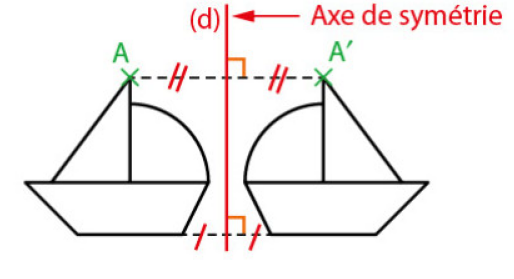
\includegraphics[scale=.8]{fig1}
	\end{center}	
\end{myex}

\begin{multicols}{2}
	
	\begin{center}
		\includegraphics*[scale=0.25]{def}
	\end{center}
	
	\begin{myprops}
		Soit $(d)$ une droite :
		\begin{itemize}
			\item Si un point $A$ n'appartient pas à la droite $(d)$, alors son symétrique par rapport à la droite $(d)$ est le point $A'$ tel que \kw{$(d)$ est la médiatrice du segment $[AA']$}.
			\item Si un point $B$ appartient à la droite $(d)$, alors son symétrique par rapport à la droite $(d)$ est lui même.
		\end{itemize}
	\end{myprops}
	
	
\end{multicols}



\section{Symétrie centrale}




\begin{mydef}

	Deux figures sont \kw{symétriques par rapport à un point $O$} si elles se superposent lorsqu'on effectue un demi-tour autour du point $O$. Le point $O$ est appelé \kw{centre de symétrie}.
	
\end{mydef}

\begin{myex}
	\begin{center}
		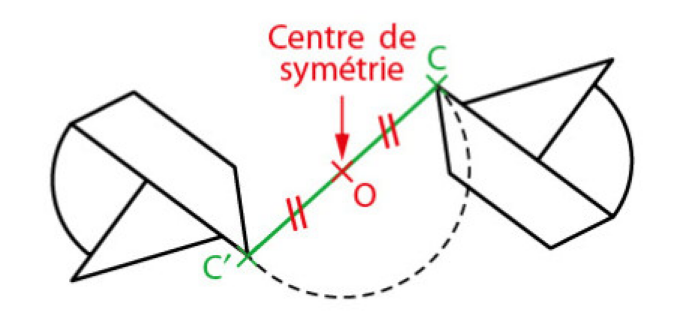
\includegraphics[scale=.75]{fig2}
	\end{center}
\end{myex}




\newpage

\section{Propriétés de la symétrie}

\begin{myprops}
	\begin{itemize}
		\item Le symétrique d'une droite par rapport à une droite ou un point est une autre droite. La symétrie \hspace*{6cm}.
		\item Si deux droites sont \kw{symétriques par rapport à un point} alors elles sont \hspace*{4cm}.
	\end{itemize}
\end{myprops}

\begin{myexs}
	\begin{multicols}{2}
		\begin{center}
			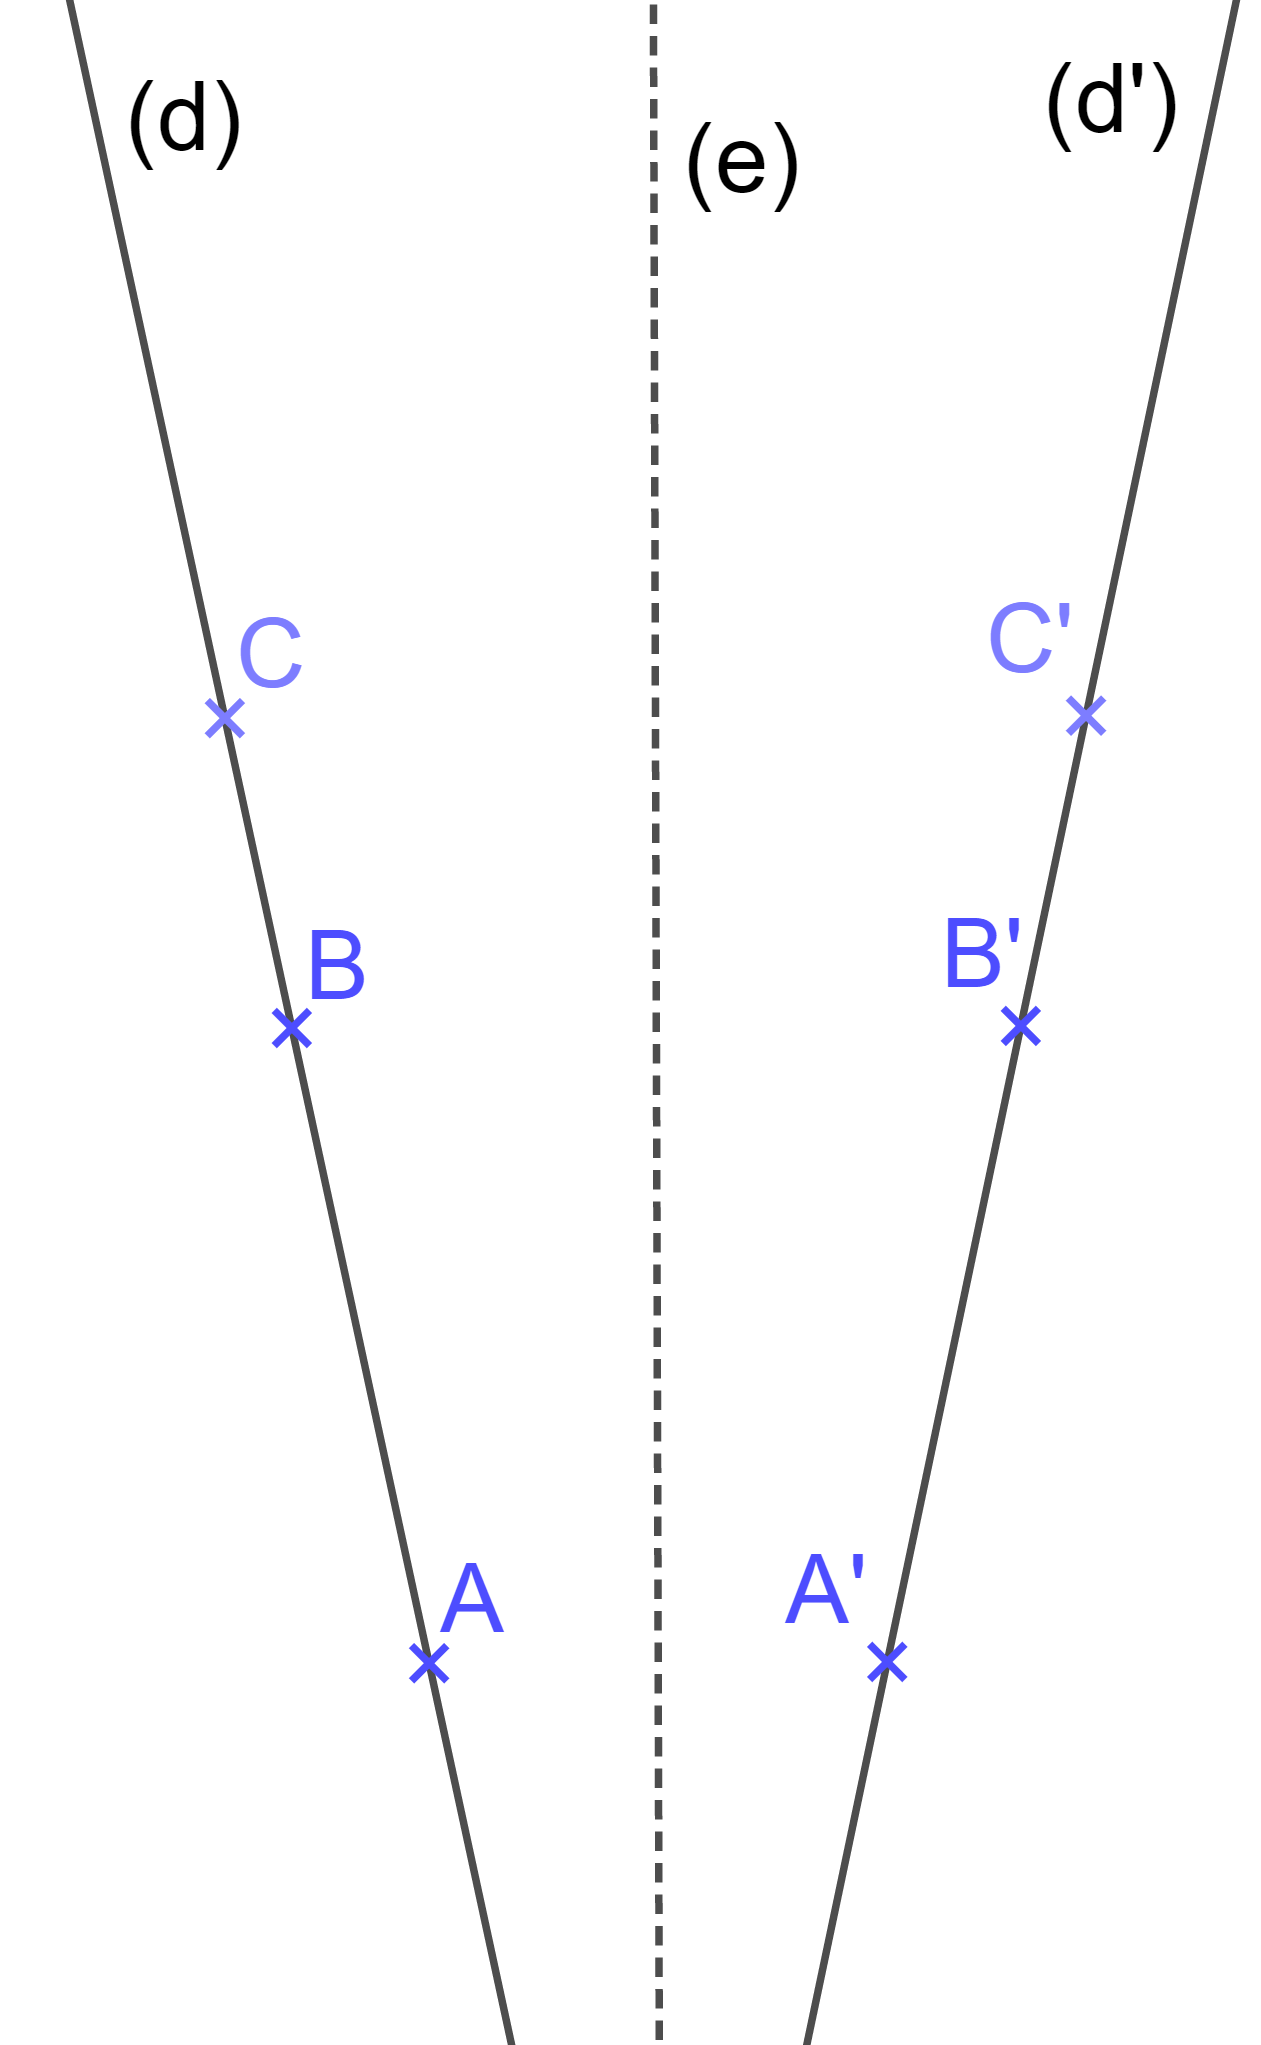
\includegraphics[scale=0.1]{sym_droites1}
		\end{center}

		\begin{itemize}
			\item Les points $A$, $B$ et $C$ sont alignés, donc $A'$, $B'$ et $C'$ leur symétriques par rapport à la droite $(e)$ sont \hspace*{6cm}
		\end{itemize}	
		
		\begin{center}
			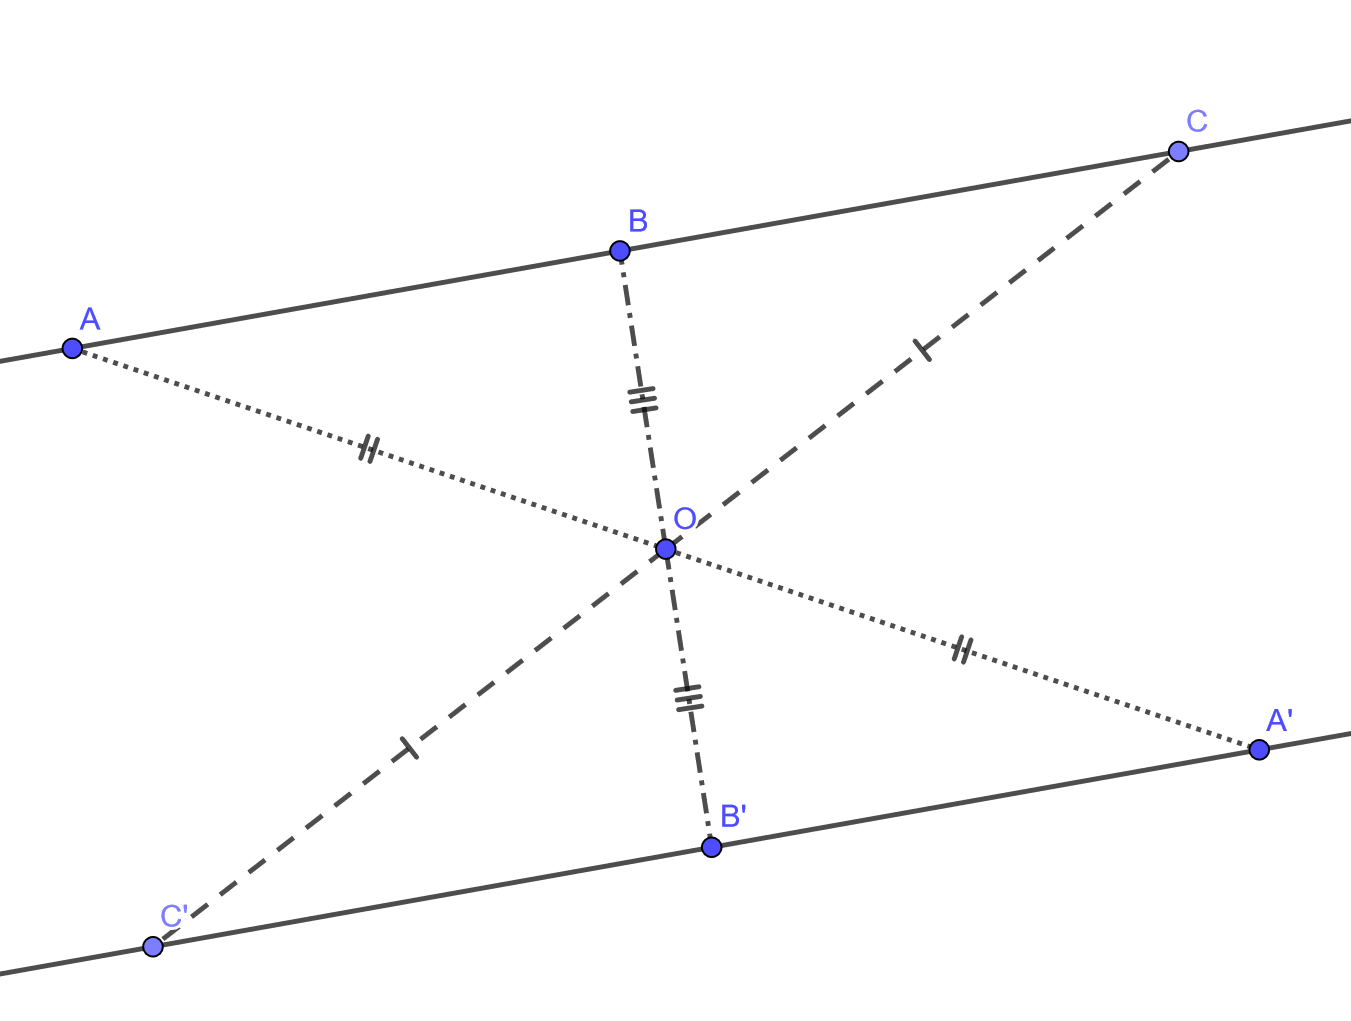
\includegraphics[scale=0.2]{sym_droites2}
		\end{center}
	
		\begin{itemize}
			\item Les points $A$, $B$ et $C$ sont alignés, donc $A'$, $B'$ et $C'$ leur symétriques par rapport à la droite $(e)$ sont \hspace*{6cm}.
			\item La droite $(AB)$ est \hspace*{4cm} \\ à la droite $(A'B')$.
		\end{itemize}
	\end{multicols}
\end{myexs}

\begin{myprop}
	Le symétrique d'un segment par rapport à une droite ou un point est un segment \hspace*{6cm} .
\end{myprop}

\begin{myex}
	\begin{center}
		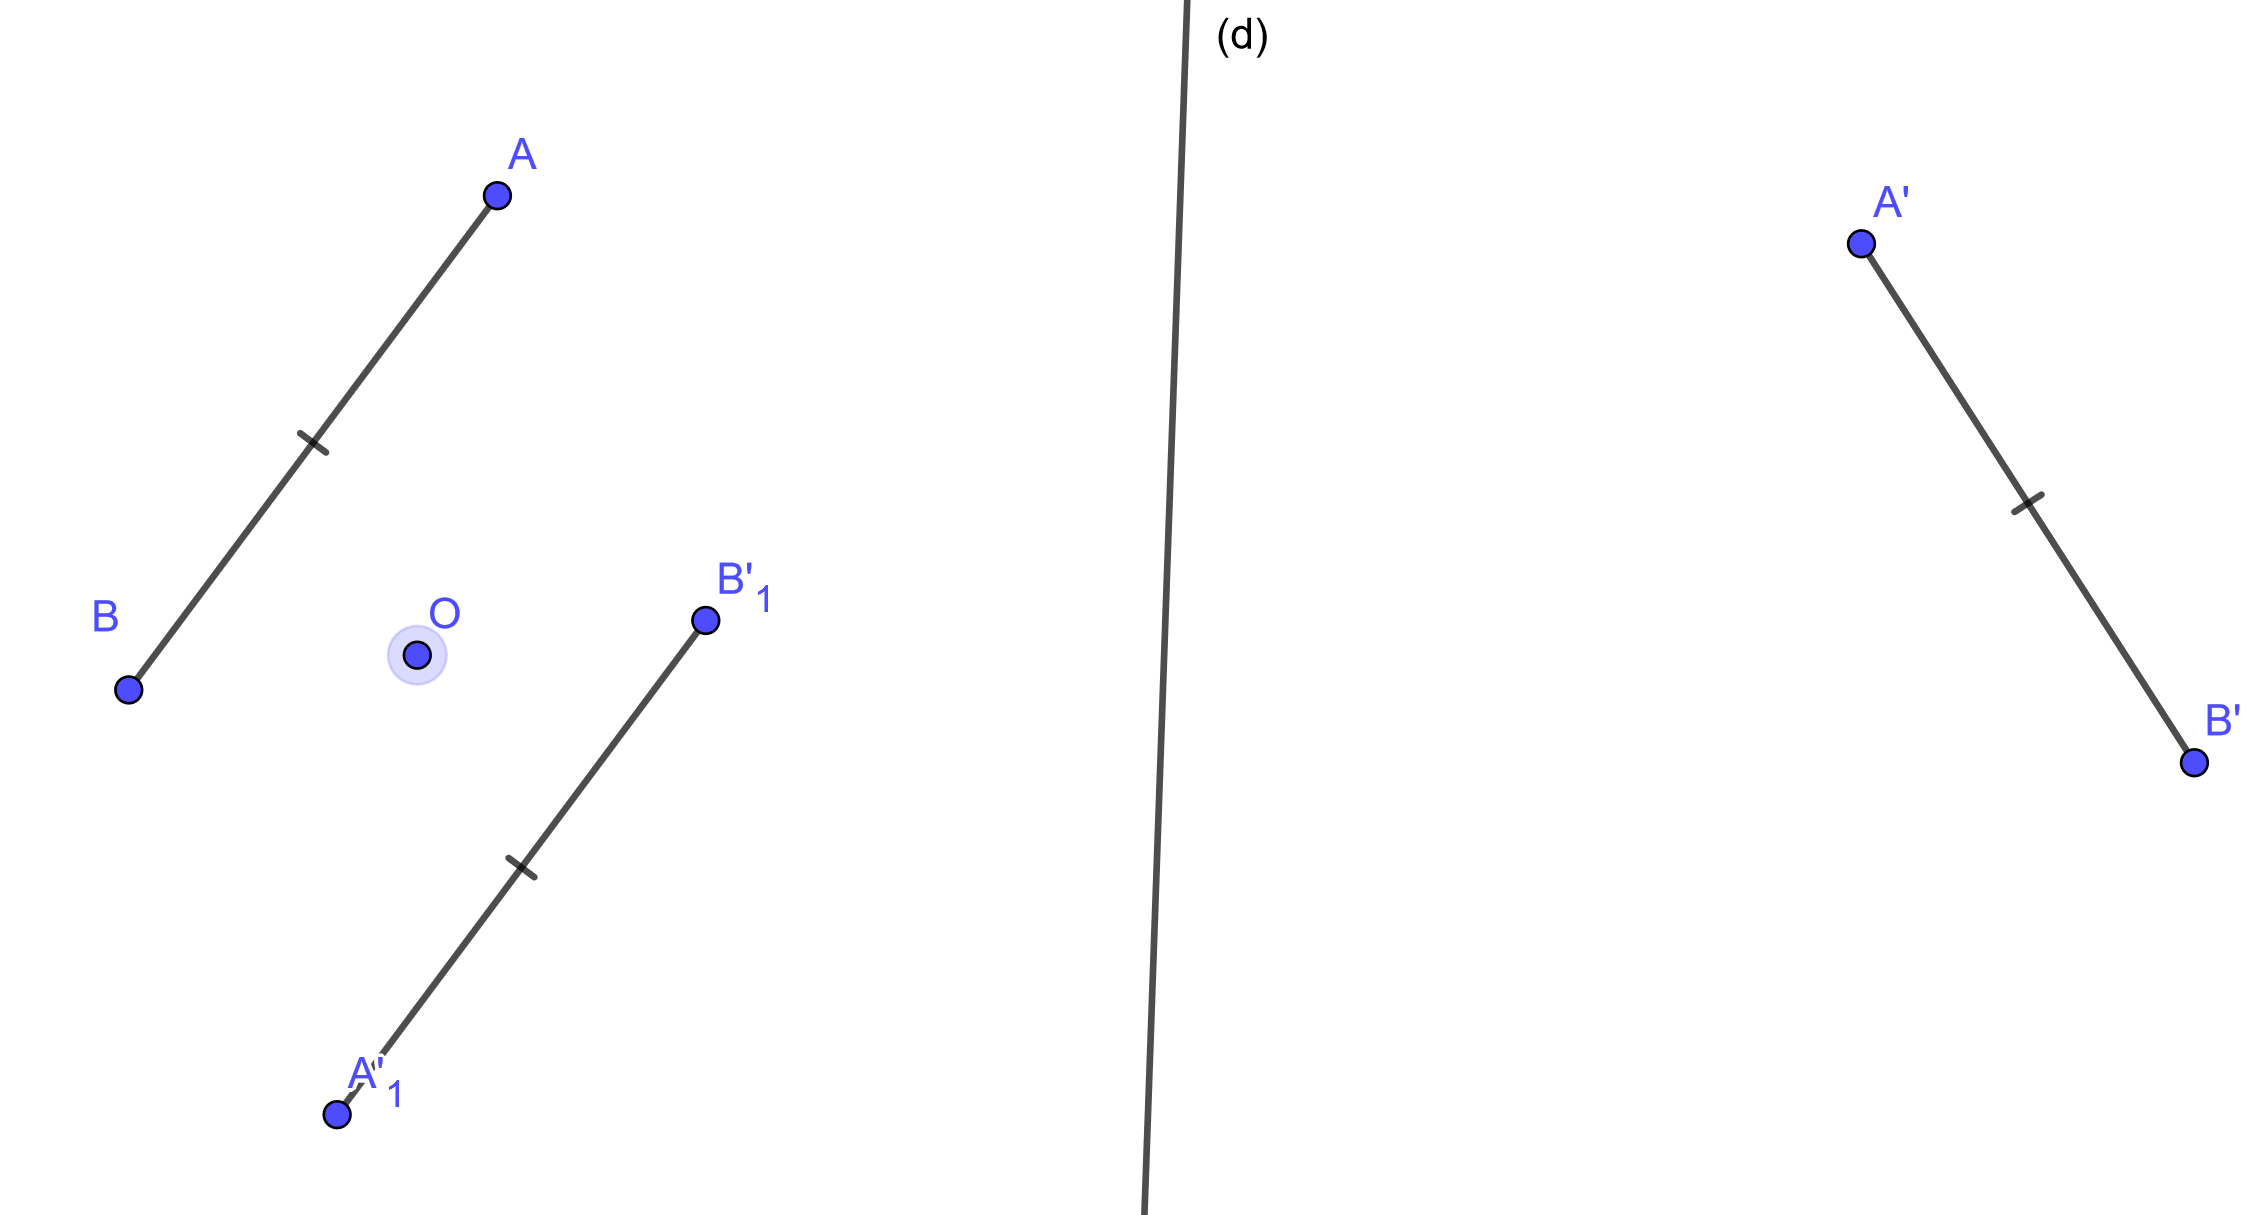
\includegraphics[scale=0.2]{sym_seg}
	\end{center}

Le segment $[A'B']$ est le symétrique du segment $[AB]$ par rapport à la droite $(d)$ et $[A'_1B'_1]$ le symétrique de $[AB]$ par rapport au point $O$. 
Ils ont tous \\

	
\end{myex}

\begin{myprop}
	Le symétrique d'une figure par rapport à une droite ou un point est une figure de même forme. La symétrie \kw{conserve \hspace*{8cm}} \\ .
\end{myprop}

\begin{myex}
	\begin{center}
		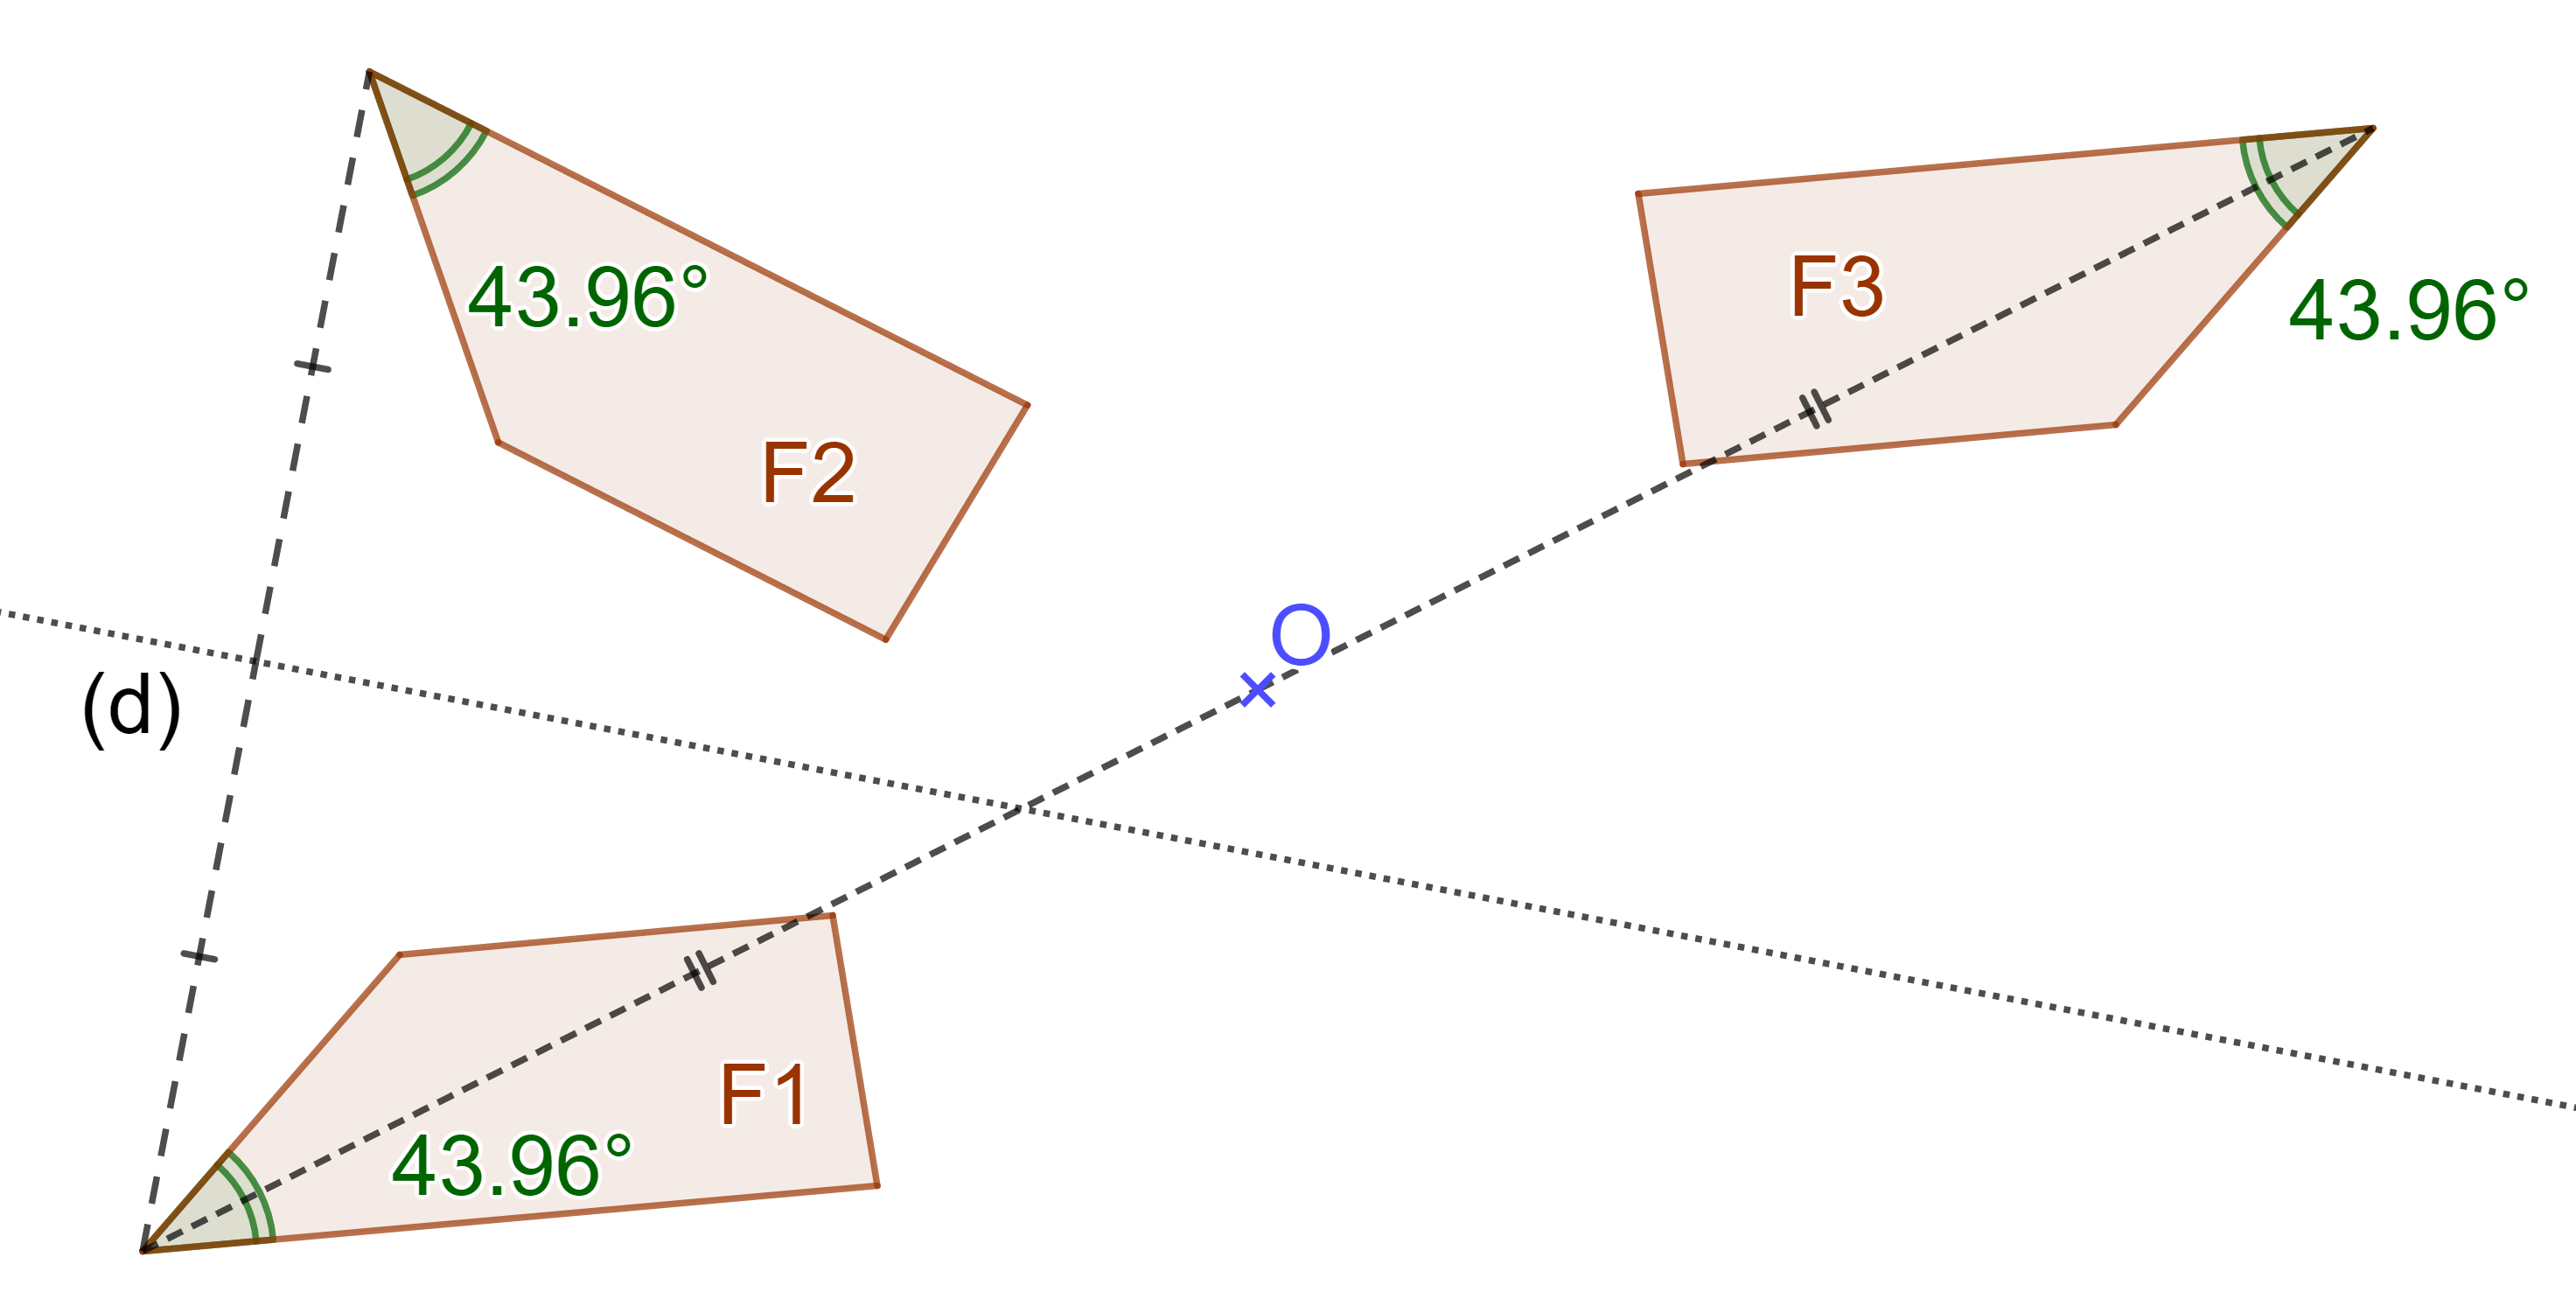
\includegraphics[scale=0.2]{sym_figures}
	\end{center}
	
	La figure $F2$ est le symétrique de $F1$ par rapport à la droite $(d)$; $F3$ est le symétrique de $F1$ par rapport au point O.
	Elles ont \\
\end{myex}




\section{Identifier un axe ou un centre de symétrie}

\section{Tableaux de proportionnalité}

\begin{center}
	\includegraphics*[scale=0.3]{tabs}
\end{center}

\begin{questions}
	\question Pour chacun des tableaux ci-dessus, dire s'il s'agit d'un tableau de proportionnalité. Justifier la réponse. 
\end{questions}
\end{document}